\cotefile{160}
\scanpage{13}
\[
 \Delta_n(\unsure{U|u}\mathbin{.}X)=(\det U)\,\Delta_n(X)\qquad\big]
\]
\inserted{$u\in\Gamma_n$}
\deleted{\unsure{autrement dit} \illegible{1} (\unsure{$U\in\Gamma_n$} \illegible{1} \unsure{ceci dit|coefficient})}

\deleted{donc les $\Delta_i=\Delta_n A_i$ sont aussi des invariants sous $S\Gamma_n$.}

\uline{Corollaire}\quad
\[
 \deleted{\mathbb F_p[X_1,\ldots,X_n]^{S\Gamma_n}\simeq
 \mathbb F_p[A_1,\ldots,\unsure{A_n|\Delta_n}]}
\]
\[
 \mathbb F_p[X_1,-,X_n]^{S\Gamma_n}
 =\mathbb F_p[A_1,\ldots,A_{n-1},\Delta_n]\quad
 \deleted{\unsure{\simeq}\ \mathbb F_p[X_1,\ldots,X_n}
\]
(et $\Gamma_n/S\Gamma_n\overset{\det}{\simeq} F_p^*$ opère sur
$\mathbb F_p[A_1,-,A_{n-1},\Delta_n]$ en laissant $A_1-A_{n-1}$ et par homothéties sur $\Delta_n$ ..

\uline{Dém} On a le diagramme commutatif
(\inserted{\unsure{flèches|flèche} $i^0$} défini par l'inclusion
$\mathbb F_p[A_1,-,A_{n-1},\unsure{\omega_n|W_n|\Delta_n}]\subset
\deleted{\mathbb F}\mathbb F_p[X_1,-,X_n]^{S\Gamma_n}$)
\diagram{\begin{tikzcd}[ampersand replacement=\&,row sep=large,column sep=large]
\mathbb E^n/\Gamma_n^{0}\arrow[r,"i^0"]\arrow[d,"p=\mathrm{can}" ] \& \mathbb E^n\arrow[d,"q"]\\
\mathbb E^n/\Gamma_n\arrow[r,"\sim"] \& \mathbb E^n
\end{tikzcd}}
$q$ définie par l'inclusion
$\mathbb F_p[A_1,-,A_{n-1},\pm\Delta_n^{p-1}]\subset
\mathbb F_p[A_1,-,A_{n-1},\Delta_n\unsure{]}$

Ainsi $p$ et $q$ sont des rev. galoisiens de groupe $\mathbb F_p^*$, identifiant le but au quotient de la source par ledit groupe, et $i^0$ est un \unsure{hom|homom.} compatible avec ces opérations, donc géom. bijectif et birationnel, donc (comme $\mathbb E^n$ est normal) un iso par le Main Theorem.
% archive sheet number: 12
\scanpage{14}
\uline{Corollaire} Soit $M\subset\mathbb G_{aS}$ un sous-groupe fini étale
\deleted{loc. libre} de rg $p^n$, d'où
$a=(a_0,\ldots,a_{n-1})\in\Gamma(S,\underline O_S)^n$ tel que
$M=\operatorname{Ker} f_a$, \inserted{$a_0$ inversible.}
On a alors une \uline{\unsure{correspondance} biunivoque}\margin{préciser} entre l'ens des structures
\uline{spéciales linéaires} (sur $\mathbb F_p$) de $M$, et l'ens des racines
$(p-1)$ièmes de $a_0$.
Ou mieux : $(\bigwedge_{\mathbb F_p}^{n} M)^*$ s'identifie à
$(\mathbb F_p^{\times})_S$-torseur des racines $(p-1)$-ièmes de $a_0$.
i.e. \deleted{à} \deleted{\unsure{image}} l'image inverse de
$a_0\in\Gamma(S,\underline O_S)^\times$ par
$\deleted{\underline O_S}G_m\mathrel{\overset{x\mapsto x^{p-1}}{\rule{1.6em}{.4pt}}}G_m$,
qui \deleted{est} un torseur sous $\mu_{p-1\, S}\simeq(\mathbb F_p^\times)_S$.

\figure{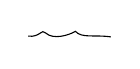
\begin{tikzpicture}\draw (0,0)..controls(.15,-.02)and(.17,.10)..(.22,.04)..controls(.32,-.05)and(.51,.01)..(.60,.06)..controls(.68,-.03)and(.84,.02)..(1.05,-.01);\end{tikzpicture}}

\uline{NB} \deleted{\unsure{La}} La donnée d'un \unsure{$p$-groupe|sous-groupe} fini étale
\deleted{\unsure{sur}} $M$ de rang $n$ sur $\mathbb F_p$, sur $S$, équivaut à la donnée de $E$ loc. libre de rg $n$, avec iso
\[
 E^{(p)}\xrightarrow{\overset{u}{\sim}}E
\]
(On prend $E\simeq M\otimes_{\mathbb F_p}\underline O_S$, on récupère $M$ comme
$\deleted{E}M=\operatorname{Ker}(\mathrm V(E)\xrightarrow{\mathrm{id}-u\circ F_E}\mathrm V(E)$.
La donnée d'un hom $M\longrightarrow\mathbb G_a$ équivaut à la donnée d'un hom
$\underline O_S$-lin. $\mathbb E\longrightarrow\underline O_S$, i.e. d'une section
\deleted{\unsure{en}} \deleted{\unsure{$\xi$}} de $\check E^{\unsure{*}}$.
Noter que $\check E$ est aussi muni d'une structure
$\check E^{(p)}\xrightarrow{\overset{\check u}{\sim}}\check E$.
% archive sheet number: 13
\scanpage{15}
Pour tte section $\unsure{\zeta|\xi}$ de $\check E$ (i.e hom $\varphi:M\to\mathbb G_a$) on peut considérer les \unsure{sections|section}
\[
 \zeta^{(p)\unsure{*|1}}\overset{\mathrm{def}}{=}
 u(\zeta^{(F)\,\to\,\text{frobénius})})
\]
et par itération les $\zeta^{(p^i)}$. Elles correspondent aux composés de
$\varphi:M\mathrel{\rule{1.3em}{.4pt}}G_a$ avec $F_{G_a}:G_a\to G_a$,
et \deleted{\unsure{leurs|les}} \inserted{ses} itérés $F_{G_a}^{i}$.

Considérons
\[
 \zeta\wedge\zeta^{(p)}\ldots\wedge\zeta^{(p^{n-1})}
 \in\Gamma(\textstyle\bigwedge^n\check E)
\]
On trouve ainsi \inserted{(en changeant de base)} une application \unsure{polynômiale|polynômial|polynomiale}
\[
 \Delta^{E}_{\unsure{M|n}}:\check E\longrightarrow\textstyle\bigwedge^n\check E
\]
homogène de degré $1+p+\text{---}+p^{\unsure{n-1}}=\frac{p^n-1}{p-1}$, d'où
\deleted{d'où \unsure{un morphisme}}
\[
 \begin{aligned}
 \Delta_{n}^E:\quad &\mathrm V(E)\longrightarrow \mathrm V(\textstyle\bigwedge^{n}E)\\
 &\hspace{.7em}\shortparallel \hspace{6em}\shortparallel\\[-2pt]
 &\mathrm W(\check E)\hspace{3.2em}\mathrm W(\textstyle\bigwedge^{n}\check E)
 \end{aligned}
\]
\deleted{\uline{Prop} \unsure{Sur} chaque fibre,}

Considérons l'image inverse dans $\mathrm V(E)$ de la section \unsure{nulles|nulle} de
$\mathrm V(\bigwedge^{n}E)$, \deleted{\unsure{soit} \illegible{1}}
c'est un diviseur de Cartier relatif, dont le complémentaire
$\mathrm V(\deleted{\unsure{\bigwedge}}E)^0$ est un ouvert \unsure{univt} sch. dense.
Si $\zeta$ est une section de cet ouvert, alors $\zeta,\zeta^{(p)}\ldots\zeta^{(p^{n-1})}$
\deleted{\unsure{forment}} une base de $\check E$, et on peut écrire
\[
 \zeta^{(p^n)}+A^E_{n-1}(\zeta)\,\zeta^{(p^{n-1})}
 \unsure{+\cdots+|-\cdots+}A^E_0(\zeta)\,\zeta=0
\]
% archive sheet number: 14
\scanpage{16}
avec des $A_i^E(\unsure{\zeta|\xi})$ $(0\leq i\leq n-1)$ \unsure{uniquemt|uniquement} déterminés.
On trouve ainsi des hom
\[
 A_i^E\in\Gamma(\mathrm V(E)^0,\deleted{\underline O_{\mathrm V(E)^0})}
 \qquad\text{i.e.}\qquad A_i^E:\mathrm V(E)^0\longrightarrow G_{aS}
\]
uniquemt déterminés par la condition précédente.
On peut les interpréter comme des éléments de
\[
 \underline{\mathrm{Sym}}^*(E)_{\Delta_n^E}
\]
\deleted{$A_i$ est homogène de degré $p$}

Ceci dit, on trouve que les $A_i$ sont des sections de $\underline{\mathrm{Sym}}(E)$, i.e. sont définis sur
$\mathrm V(E)$ tt entier, bien entendu ils y sont caractérisés par l'identité précédente.
\deleted{\unsure{$p^{n}$} \unsure{est}}

On a \unsure{encore|même}
\[
 A_0^E=(\Delta_n^E)^{p-1}\deleted{(\unsure{-1})^n}(\pm1)
\]
[celà a un sens, grâce à :
\[
 \begin{aligned}
 &(\textstyle\bigwedge^n\check E)^{p-1}\simeq\underline O_S\\
 \text{i.e.}\quad&(\textstyle\bigwedge^n\check E)^p=\textstyle\bigwedge^n\check E^{(p)}\simeq
 (\textstyle\bigwedge^n\check E)\quad\big]
 \end{aligned}
\]

\uline{NB} Supposons que $\zeta$ est une section de $\mathrm V(E)^0$, \deleted{Alors}
donc les $\zeta^{p^i}$ $(0\leq i\leq n-1)$ font une base de $\check E$, qui s'identifie donc à
$\underline O_S^{n}$, avec la \deleted{\unsure{loi|forme|choix}} de \unsure{puiss.} \unsure{$p$ième}
$e_0^{(p)}=e_1,e_1^{(p)}=e_2,\ldots,e_{n-2}^{(p)}=e_{n-1}$, et
% archive sheet number: 15
\scanpage{17}
\[
 e_{n-1}^{(p)}=-\bigl(\underbrace{A_0(\unsure{\zeta|\xi})}_{a_0}e_0+
 \text{---}+\underbrace{A_{n-1}(\zeta)}_{a_{n-1}}e_{n-1}\bigr)
\]
i.e. on trouve la matrice
\[
 \begin{pmatrix}
 0&0&&0&-a_0\\
 1&0&&0&\unsure{-a_1|a_1}\\
 0&1&\ddots&\vdots&\\
 \bar 0&\bar 0&\cdots&\bar 0&\\
 0&0&\ddots&1&\\
 0&0&&0&-a_{n-1}
 \end{pmatrix}
\]
pour l'application de puiss. \unsure{$p$ième}. Ainsi \deleted{On}
\deleted{\unsure{donnée de}} \inserted{\uline{retrouve que}} la donnée
\deleted{\unsure{du}} d'un sous- \textemdash\textemdash

\diagram{\scriptsize\begin{tikzcd}[ampersand replacement=\&,column sep=small,row sep=large]
 (a_0,-\,a_{n-1})\quad a_0\ \text{inv}
 \arrow[d,<->] \& \subset \&
 (a_0,-,a_{\unsure{n|n-1}})\arrow[d,<->]\\
 \begin{array}{l}\text{ss-gpes }\deleted{\unsure{f}}\text{finis étales de }G_a\end{array}
 \arrow[d,<->] \& \subset \&
 \begin{array}{l}\text{ss-groupes finis loc.}\\\text{libres de rg }p^n\text{ de }G_a\end{array}
 \arrow[d,<->,"?"]\\
 \begin{array}{l}\deleted{E}F\text{ loc. libre }\inserted{\mathrm{rg}\,n}\text{ avec }
 {\deleted{E}F}^{(p)}\simeq\deleted{E}F,\\
 \text{et section }\zeta\text{ de }\deleted{E}F\text{ avec}\\
 \zeta,\zeta^{(p)}\ldots\zeta^{(p^{n-1})}\text{ une base}
 \end{array}
 \arrow[uu,<->,bend right=48] \& \subset \&
 \begin{array}{l}F\text{ loc. libre rg }n\text{ avec}\\
 {\deleted{\unsure{E}}F}^{(p)}\to F\ \text{(pas néc. iso)}\\
 \text{et }\zeta\in\Gamma F\text{ telle que}\\
 \zeta,\zeta^{(p)}\text{---}\zeta^{(p^{n-1})}\text{ base}
 \end{array}
 \arrow[uu,<->,bend right=50,"{\text{\unsure{trivial|trivial\,?}}}"]
\end{tikzcd}}
% archive sheet number: 16
\scanpage{19}
\diagram{\begin{tikzcd}[ampersand replacement=\&,row sep=small]
 X'\arrow[d]\\
 X\quad\text{déduit de }X'\text{ en ``pinçant'' }a\text{ et }b
\end{tikzcd}}
\[
 \begin{aligned}
 H&\subset\mathbb G_{aX}=\operatorname{Ker}
 \bigl(G_{aX}\xrightarrow{x^{p^n}+c_{n-1}x^{p^{n-1}}\ \text{---}\ c_0x}G_{aX}\bigr)\\
 H'&\subset\mathbb G_{aX'}\qquad H'_a\deleted{\unsure{(a)}}=H'_b\qquad
 c_i(\unsure{a})=c_i(b)
 \end{aligned}
\]
\diagram{\begin{tikzcd}[ampersand replacement=\&,row sep=small,column sep=small]
 \bullet\arrow[r,dash] \& H\arrow[r] \& G_{aX}\arrow[r]\arrow[dr,"\varphi"] \&
 G_{aX}\arrow[r,dash]\arrow[d,dotted,"\hat\psi"] \& \bullet\\
 \&\&\&G_{aX}\&
\end{tikzcd}}
$\varphi\mid\hat H=0$ i.e. $\hat\varphi$ se
\deleted{\unsure{pro}} \inserted{\unsure{factorise|factor.}} en $\Psi$.
\[
 (\operatorname{Ker}\varphi')_{\unsure{y'|\eta'}}=(\operatorname{Ker}\varphi)_y=N'_y
 \qquad \overline N_y=N'
\]
\inserted{adh. sch. dans $G_{aX'}$}

$N'\subset H'\qquad\hat N'\simeq\hat H'$ i.e. $G_{aX'}/N'\longrightarrow G_{aX'}$ \uline{étale}

\uline{Mais} supposons $N'(a)\ne N'(b)$
\[
 \begin{aligned}
 \overset{\swarrow}{N'}&\subset H'\subset G_{aX'}\\
 H'(a)&=H'(b)\qquad \hat N'\simeq\hat H'\quad\text{i.e.}\quad
 G_{aX'}/\deleted{N'}\mathrel{\unsure{\rule{1.3em}{.4pt}|\to}}G_{aX'}/H'\quad\text{étale}\\
 N'(a)&\ne N'(b)
 \end{aligned}
\]
\diagram{\scriptsize\begin{tikzcd}[ampersand replacement=\&,row sep=large,column sep=small]
 \bullet\arrow[r]\&N'\arrow[r,dash]\&G_{aX'}\arrow[r,"f_{\alpha'}"]\&
 G_{aX'}\arrow[r]\arrow[d,equal]\arrow[rr,bend left=24,"{u_{\lambda'}\ \text{(homothétie)}}"]
 \&0\&G_{aX}\\
 \&\bullet\arrow[r,dash]\&\underset{\text{étale}}{\unsure{K_0'|K'}}\arrow[r]\&
 G_{aX'}\arrow[r,"f_{\beta'}"]\arrow[dr,"u_{\lambda'}"']\&
 G_{aX'}\arrow[r,dash]\arrow[d,dotted,"{\deleted{\unsure{\xi|\exists}}\Psi}"]\&0\\
 \&\&\&\&\unsure{G_a|\mathbb G_a}\&
\end{tikzcd}}
$\unsure{\big\}|d)}\quad u_{\lambda'}f_{\alpha'}$\inserted{$=\lambda'f_{\alpha'}$}
\unsure{passe|pour} à $X$ \deleted{\unsure{i.e.} \unsure{$\lambda'f_\alpha$} \unsure{passe à $X$}}
% archive sheet number: 18
\scanpage{20}
\deleted{\unsure{symétrique} \unsure{additif}}
\figure{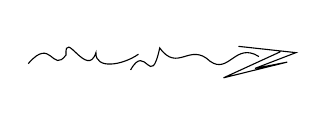
\begin{tikzpicture}[x=1cm,y=1cm]
\draw (0,0) .. controls (.3,.35) and (.3,-.13) .. (.48,.11)
 .. controls (.46,.45) and (.75,-.2) .. (.86,.14)
 .. controls (.85,-.08) and (1.2,-.02) .. (1.4,.12);
\draw (1.3,-.08) .. controls (1.5,.28) and (1.55,-.35) .. (1.67,.2)
 .. controls (1.9,-.12) and (2.05,.28) .. (2.31,.03)
 .. controls (2.55,-.14) and (2.63,.28) .. (2.93,.09);
\draw (2.67,.22)--(3.40,.14)--(2.88,-.06)--(3.29,.02)--(2.48,-.18)--(3.20,.15);
\end{tikzpicture}}
\[
 \begin{aligned}
 X^p+A_1(X_1,-,X_n)X^{p^{n-2}}+A_2(X_{\unsure{2|1}},-\,X_n)X^{p^{n-3}}\ \text{---}\\
 {}+A_{n-1}(X_1,-X_n)X
 \end{aligned}
\]

% margin note written sideways
\margin{\scriptsize
$H_0\quad G_0\quad K_0=G_0/H_0$

$G/\bar H_0=\bar G_0/\bar H_0=\bar K_0$

$G/H=K$
\diagram{\resizebox{\marginparwidth}{!}{\begin{tikzcd}[ampersand replacement=\&,column sep=small,row sep=small]
G_0\arrow[r]\&K_0\arrow[r,"\unsure{=|\sim|\Rightarrow}"]\&K_0\\
G\arrow[r,"{\deleted{\unsure{K}}}"]\&\bar K_0\arrow[r,"?"]\&\bar K\\
\&G/H\arrow[u,equal]\&
\end{tikzcd}}}
\diagram{\resizebox{\marginparwidth}{!}{\begin{tikzcd}[ampersand replacement=\&,row sep=tiny,column sep=small]
{}\arrow[r,dash]\&H_0\arrow[r,dash]\&G_0\arrow[r,dash]\&K_0^{\unsure{r|0}}\arrow[r]\&0\\
\&\&\&\unsure{\varepsilon|\xi}\arrow[u,"{\unsure{f}}"]\&\\
\&\&\&K_0\arrow[u]\&\\
\&\&\&\bullet\arrow[u,dash]\&
\end{tikzcd}}}
$\underbrace{\hphantom{G_0\quad K_0\quad0}}$

$\operatorname{Hom}(\alpha_{p^r},G_a)$

$\shortparallel$

$\operatorname{Hom}(\alpha_{p^r},\alpha_{p^r})$

$V=0,\ F^r=0\quad p=\unsure{0|\bullet}$

$\mathbb F_p(\unsure{F|E|\mathbb F})/F^r$}

\[
 \begin{aligned}
 X_1\check e_1+\text{---}+X_n\check e_n\\
 X_1^p\check e_1\qquad X_n^p\check e_n\\
 X_1^{p^{n-1}}\check e_1\qquad X_n^{p^{n-1}}\check e_n
 \qquad&\lambda^{1+p+\text{---}\,p}\\
 X_1^{p^n}\check e_1\qquad X_n^{p^n}\check e_n
 \qquad&\lambda^{p^n-p^{n-1}}\quad\lambda^{p^n-p^{n-2}}
 \end{aligned}
\]
\[
 X_1^{p^n}+a_1X_1^{p^{n-1}}+a_2X_1^{p^{\unsure{n-1|n-2}}}\ \text{---}
 +a_nX_1=0
\]
\figure{
\begin{tikzpicture}[x=1cm,y=1cm]
\draw (0,.25) .. controls (.06,-.25) and (.31,-.11) .. (.21,.17)
 .. controls (.20,.35) and (.14,-.16) .. (.41,-.04);
\foreach \x in {.40,.55,.70,.85,1.0}
 {\draw (\x,-.04) .. controls (\x+.21,.00) and (\x+.03,.34) .. (\x+.01,.16)
 .. controls (\x-.04,-.04) and (\x+.08,-.13) .. (\x+.17,-.02);}
\draw (1.15,-.02)..controls(1.35,.02)and(1.32,-.13)..(1.49,.02);
\end{tikzpicture}}
\[
 {f}^{p^{\unsure{n}}}+a_1 f^{p^{n-1}}\ \text{---}
 +a_{n-1}f^{\unsure{p}}+a_n f=0
\]
\figure{\begin{tikzpicture}[x=.55cm,y=.55cm]
\draw (0,0)..controls(.50,.12)and(.04,.72)..(.34,.69)
 ..controls(.82,.63)and(.17,1.28)..(.56,1.12)--(.91,.95);
\end{tikzpicture}}
\[
 \begin{aligned}
 f&\quad f^p\quad\text{---}\quad f^{p^{n-1}}\\
 e_1&\quad e_2\hspace{4.2em}e_n
 \end{aligned}
\]
\[
 \begin{aligned}
 e_1^{(p)}&\longmapsto e_2\\
 e_2^{(\unsure{p|n})}&\longmapsto e_3\\[-3pt]
 &\cdots\\
 e_{n-1}^{(p)}&\longmapsto e_n\\
 e_n^{(p)}&\mathrel{\unsure{\rule{1.3em}{.4pt}|\mapsto}}a_1 e_n+a_2 e_{n-1}\ \text{---}+a_{\text{\uuline{$n$}}}e_1\\
 &a_n\ne0
 \end{aligned}
\]
\figure{\begin{tikzpicture}[x=.55cm,y=.55cm]
\draw (0,0)..controls(.40,.04)and(.0,.65)..(.37,1.03)
 ..controls(.72,1.5)and(.20,1.95)..(.64,1.90)
 ..controls(1.13,1.78)and(.55,2.39)..(.93,2.27)
 ..controls(1.26,2.15)and(.70,2.57)..(1.13,2.45);
\end{tikzpicture}}
\[
 \begin{aligned}
 e_1^p=e_2\quad e_2^p=e_3\ \text{---}\quad e_{n-1}^{p}=e_n,\quad
 e_n^p={}&-(\unsure{a_1}e_n+a_2e_{n-1}\\
 &{}+a_ne_1)
 \end{aligned}
\]
\[
 \begin{aligned}
 \underset{\text{loc. \unsure{li.|l.|lib.} t.f.}}M\qquad&M^{(p)}\xrightarrow{\sim}M
   \qquad\underline M\longrightarrow\underline O\\
 &e_1\ \text{--}\ e_n\qquad e_i^p\mathrel{\unsure{\rule{1.3em}{.4pt}|\to|\mapsto}}\sum_j\lambda_{ij}e_j
 \end{aligned}
\]
\[
 M\to M^{(p)}\longrightarrow\underline M\qquad \unsure{x^p|xp}
\]
% archive sheet number: 19
\scanpage{21}
\[
 (f^{p-1}-g^{p-1})X^{p^{\unsure{2}}}-
 (f^{p^2-1}-g^{p^2-1})X^p+
 (f^{p^2-1}g^{p-1}-g^{p^2-1}f^{p-1})X
\]
\figure{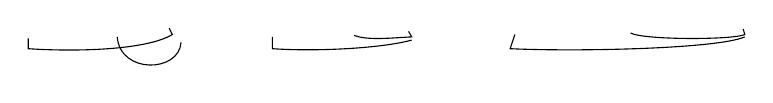
\begin{tikzpicture}[x=1cm,y=1cm]
\draw (0,0)--(0,-.13)..controls(.6,-.17)and(1.5,-.15)..(1.83,.05)--(1.79,.13);
\draw (1.13,.02)..controls(1.17,-.46)and(1.92,-.43)..(1.94,-.05);
\draw (3.1,.02)--(3.1,-.13)..controls(3.7,-.17)and(4.52,-.12)..(4.87,-.02);
\draw (4.14,.04)..controls(4.30,-.03)and(4.65,.01)..(4.87,.02)--(4.83,.09);
\draw (6.18,.05)--(6.12,-.13)..controls(7,-.17)and(8.76,-.13)..(9.10,.02);
\draw (7.65,.07)..controls(7.8,-.02)and(8.95,-.02)..(9.10,.05)--(9.08,.12);
\end{tikzpicture}}
\[
 \begin{aligned}
 f^{p^3}+a f^{p^2}+b f^p+c f&=0\\
 g^{p^3}+a g^{p^2}+b g^p\unsure{+|-}c g&=0\\
 h^{p^3}+a h^{p^2}+b h^p+\unsure{c}h&=0
 \end{aligned}
\]
\[
 \det\begin{pmatrix}
 X_1^{p^{n-1}}&\text{---}&X_1^p&X_1\\[1.6ex]
 X_n^{p^{n-1}}&&X_n^p&X_n
 \end{pmatrix}
 \qquad 1+p+\text{---}+p^{n-1}=\frac{p^n-1}{p-1}
\]
\[
 \deleted{\unsure{X_1}\,\unsure{X_2}\,\unsure{X_n}}
 \prod_{\substack{\unsure{\mathbb P^{n-1}|\mathrm P^{n-1}|\mathbb P^n}(\mathbb F_p)\\
 (\lambda_1\ \text{--}\ \lambda_n)}}(\lambda_1X_1+\text{---}+\lambda_nX_n)
\]
\[
 \prod_{i=1}^{n}\prod_{\lambda\in\mathbb F_p^{n-i}}
 (X_i+\lambda_1 X_{\unsure{i+1|i-1}}\ \text{---}+\lambda_{n-i}X_n)
\]
\[
 \begin{aligned}
 x^{p^2}y^p-y^{p^2}x^p&\qquad x^{p^2}y-y^{p^2}x\\
 \frac{(x^p y-y^p x)^p}{x^p y-y^p x}&=(x^p y-y^p x)^{p-1}\\
 & (x\,y\\
 &\left(\frac{x}{y}\right)^{p^{\unsure{2}}}-\frac{x}{y}\unsure{=|-}
 \end{aligned}
\]
% archive sheet number: 20
\scanpage{22}
\[
 \begin{aligned}
 &\alpha\qquad\beta\\
 &x^{p^2}+ax^p+bx\\
 &\alpha^{p^2}+a\alpha^p+b\alpha=0\\
 &\beta^{p^2}+a\beta^p+b\beta=0
 \end{aligned}
\]
\[
 \begin{aligned}
 a(\alpha^p\beta-\beta^p\alpha)&=-(\alpha^{p^2}\beta-\beta^{p^2}\alpha)\\
 a&=-\frac{\alpha^{p^2}\beta-\beta^{p^2}\alpha}{\alpha^p\beta-\beta^p\alpha}\\
 b&=\frac{\alpha^{p^2}\beta^p-\beta^{p^2}\alpha^p}
 {\alpha^p\beta^{\deleted{\unsure{p}}}-\beta^p\alpha^{\deleted{\unsure{p}}}}
 \end{aligned}
\]
\[
 a(\alpha^p-\beta^p)=-(\alpha^{p^2}-\beta^{p^2})
\]
\[
 \left\{\begin{aligned}
 a&=-(\alpha-\beta)^{p^2-p}\\
 b&=-\alpha^{p^2}+\alpha^p(\alpha-\beta)^{p^2-p}
 \end{aligned}\right.
\]
\[
 \begin{aligned}
 (\alpha-\beta)^p b
 &=-\deleted{\alpha^{p^2+p}}+\beta^p\alpha^{p^2}
    +\deleted{\alpha^{p^2\unsure{-|+}p}}-\alpha^p\beta^{p^2}\\
 &=\alpha^p\beta^p(\alpha^{p^2-p}-\beta^{p^2-\unsure{1|p}})\\
 b&=\left(\frac{\alpha^{\deleted{\unsure{p}}}\beta}{\alpha-\beta}\right)^p
       (\alpha^{p^2-p}-\beta^{p^2-p})
 \end{aligned}
\]
\[
 \begin{aligned}
 &(\alpha-\beta)^p x^{p^2}\deleted{\unsure{+}}\unsure{-}(\alpha-\beta)^{p^2}x^p+
 (\alpha\beta)^p(\alpha^{p^2-p}-\beta^{p^2-p})\\
 &(\alpha^p-\beta^p)(x^{p^2}-(\alpha^{p^2}-\beta^{p^2})x^p+
 \alpha^p\beta^p(\alpha^{p^2-p}-\beta^{p^2-p})
 \end{aligned}
\]
\figure{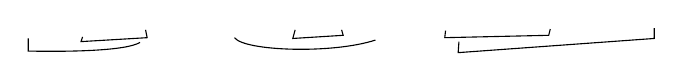
\begin{tikzpicture}[x=1cm,y=1cm]
\draw (0,0)--(0,-.16)..controls(.5,-.17)and(1.24,-.16)..(1.42,-.05);
\draw (.69,.02)--(.67,-.04)--(1.51,.01)--(1.49,.11);
\draw (2.62,.01)..controls(2.74,-.16)and(3.86,-.2)..(4.41,-.02);
\draw (3.39,.11)--(3.36,0)--(4.00,.04)--(3.98,.11);
\draw (5.30,.10)--(5.29,.01)--(6.61,.04)--(6.63,.12);
\draw (5.47,-.04)--(5.46,-.18)--(7.95,.0)--(7.95,.13);
\end{tikzpicture}}
\[
 \begin{array}{ccc}
 \lambda(f^p-g^p)&-\lambda(f^{p^2}-g^{p^2})&
 \lambda(f^{p^2}g^{\unsure{p}}-g^{p^2}f^p)\\
 0-\beta^p&0-\beta^{p^2}&0\\
 \alpha^p-0&\alpha^{p^2}&0
 \end{array}
\]
\[
 \alpha^p+\beta^p=0
\]
\[
 X\longmapsto\underbrace{\lambda(f^p-g^p)}_{r}X^{p^2}
 -\underbrace{\lambda(f^{p^2}-g^{p^2})}_{s}X^p
 +\underbrace{\lambda(f^{p^2}g^p-g^{p^2}f^p)}_{t}X
\]
\diagram{\begin{tikzcd}[ampersand replacement=\&,row sep=small]
 H\subset G_a\arrow[r,"{X\mapsto rX^{p^2}+sX^p+t}"]\arrow[d]\&G_a\\
 G_a/H\&
\end{tikzcd}}
\[
 ({\deleted{\unsure{\alpha}}f}^p\deleted{\unsure{\beta}}g
 -{\deleted{\unsure{\beta}}g}^p\deleted{\unsure{\alpha}}f)X^{p^2}
 -({\deleted{\unsure{\alpha}}f}^{p^2}\deleted{\unsure{\beta}}g
 -{\deleted{\unsure{\beta}}g}^{p^2}\deleted{\unsure{\alpha}}f)X^p
 +({\deleted{\unsure{\alpha}}f}^{p^2}{\deleted{\unsure{\beta}}g}^p
 -{\deleted{\unsure{\beta}}g}^{p^2}{\deleted{\unsure{\alpha}}f}^p)X
\]
% archive sheet number: 21
\scanpage{23}
\[
 \begin{aligned}
 f\quad g\qquad &f(a)=0&g(a)&=1\\
 &f(b)=1&g(b)&=0
 \end{aligned}
\]
$f$ et $g$ \inserted{donc} non ctes, \deleted{\unsure{f}} lin. indép. sur \unsure{$k$|$\mathbb F_p$}.
\unsure{sps} $f,g$ lin. indép. sur $\mathbb F_p$ en chaque pt sauf $a,b$

\[
 \begin{aligned}
 G_a&\supset H_f& H&=H_f\times H_g\hookrightarrow G_a\\
 &\supset H_g\\
 &&H_a&\simeq\alpha_p\times\mathbb Z/p\simeq K\hookrightarrow G_a\\
 H'&\subset\mathbb G_a&H_b&\simeq\mathbb Z/p\times\alpha_p\simeq K\hookrightarrow G_a
 \end{aligned}
\]
\[
 X\longrightarrow\deleted{\unsure{X|X'}}X'
\]
\inserted{déduit de $X$ en recollant $a,b$}
\diagram{\begin{tikzcd}[ampersand replacement=\&,row sep=small]
 H'\subset G_a\arrow[d,"\lambda"]\\ G_a
\end{tikzcd}}
\[
 \left.\begin{aligned}
 \lambda(a)&=\lambda(b)=0\\
 \lambda&\ \text{non cte}
 \end{aligned}\right\}
 \qquad H_a\simeq H_b\qquad :\alpha_p\times\mathbb F_p\alpha\times\mathbb F_p
\]
\figure{\begin{tikzpicture}[x=1cm,y=1cm]
\draw (0,.27)..controls(1.4,.17)and(2.85,-.04)..(3.74,-.07)
 ..controls(3.82,-.09)and(3.73,-.34)..(3.84,-.35)
 ..controls(5.9,-.52)and(7.62,-.33)..(8.8,-.41);
\end{tikzpicture}}
% Remaining writing is rotated 180 degrees relative to the block above.
\[
 \begin{aligned}
 &\unsure{\gamma|r}(\lambda^p-f^{p-1}\lambda)^p-\gamma^{p\deleted{\unsure{\ne}}}(\lambda^p-f^{p-1}\lambda)
 \ \big|\ \left(\frac{\lambda}{f}\right)^p-\frac{\lambda}{f}\qquad\lambda^p-f^{p-1}\lambda\\
 &\deleted{\unsure{\lambda}(\lambda^p-f^{p-1}\lambda)^p}\\
 &\gamma\lambda^{p^2}-\unsure{\gamma}f^{\unsure{p(p-1)}}\lambda^p
 \qquad\gamma=(\deleted{\unsure{f/g|g/f}})^{p}-f^{p-1}g\\
 &a\quad b\qquad\qquad
 \left(\underbrace{\left(\frac{\lambda}{f}\right)^p-\frac{\lambda}{f}}_{\unsure{\sigma|r}}\right)^{p}
 -\big(\hphantom{xx}\big)
 \end{aligned}
\]
\diagram{\begin{tikzcd}[ampersand replacement=\&,row sep=small,column sep=small]
 H\subset G_a\arrow[d,equal]\arrow[rr,dash]\&\&\text{fini plat}\\
 H_1\arrow[d,dash]\&{}\times H_2\arrow[d,dash]\&{}\times K\arrow[d,dash]\\
 \text{étale sauf en }a\&\text{étale sauf en }b\&\text{étale}
\end{tikzcd}}
\[
 H_{1a}\simeq H_{2b}\simeq\alpha_p
\]
\[
 \begin{aligned}
 f(a)&=0&g(b)&=0\\
 f(b)&=\alpha&g(a)&=\beta
 \end{aligned}
\]
$\alpha$ et $\beta$ lin. indép. sur $\mathbb F_p$
\[
 \underset{\rule{6.0em}{.35pt}}{\overset{\rule{2.8em}{.35pt}}{\alpha_p+\mathbb F_p}\alpha+\mathbb F_p}\beta
\]
$H'\subset\mathbb G_{aX'}\qquad f,g,h,$ lin. \unsure{in.|inv.} ind. sur $\mathbb F_p$
% slanted
\margin{\unsure{val.|vect.} lin. ind. en \unsure{ts} les pts sauf $a,b$}
\[
 \begin{aligned}
 i_a(H'_a)=i_b(H'_b)&=\alpha_p+\mathbb F_p\alpha+\mathbb F_p\beta\subset G_a\\
 h(a)\mathbin{;}h(b)&\in\mathbb F_p\alpha+\mathbb F_p\beta
 \end{aligned}
\]
\[
 \begin{aligned}
 \deleted{g(a),h(a)}\quad &h(a)\notin\mathbb F_p\beta
       &\text{p.ex.}\quad h(a)&=\alpha\\
 \deleted{\unsure{H_1\times H_2}}\quad &h(b)\notin\mathbb F_p\alpha
       & h(b)&=\beta
 \end{aligned}
\]
\[
 H\subset G_{aX}\qquad i_a(H_{\unsure{a|x}})\simeq\alpha_p+\mathbb F_p\alpha+\mathbb F_p\beta
 \qquad G_a
\]
\diagram{\begin{tikzcd}[ampersand replacement=\&,row sep=small,column sep=large]
 \operatorname{Ker}\varphi=H\hookrightarrow\mathbb G_a\arrow[r,"\varphi"]\arrow[dr,"u"']
 \&G_a\arrow[d,dotted,bend left=30,"?"]\\
 \&\deleted{\unsure{\lambda(a)=\lambda(b)|(H_2)}}G_a\arrow[u]
\end{tikzcd}}
\[
 G_{aX'} / H_1\times H_2\qquad
 \begin{aligned}
 \lambda&\longmapsto(\lambda/f)^p-(\lambda/f)\\
 \lambda&\longmapsto\lambda^p-f^{p-1}\lambda
 \end{aligned}
\]
% archive sheet number: 22
